\chapter{Introdución}
\label{chap:introducion}

\lettrine{N}{esta} introdución contextualízase o traballo realizado mediante a presentación do
problema abordado, dos obxectivos perseguidos e da metodoloxía xeral empregada. O propósito deste
capítulo é ofrecer unha visión global do proxecto e establecer as bases dos capítulos seguintes,
nos que se detallarán os aspectos técnicos e os resultados obtidos.

\section{Contextualización e xustificación}
Comprender e cuantificar os danos causados ás algas mariñas constitúe un paso esencial para a
investigación e a conservación dos ecosistemas submariños. A análise deste tipo de danos permite
avaliar o estado das propias algas e, ao mesmo tempo, obter información indirecta sobre a presión de
depredación herbívora e sobre o comportamento alimentario das especies que interactúan con elas.
Neste ámbito, especialistas en disciplinas como a bioloxía mariña deben examinar as mostras e
determinar tanto a intensidade do dano observado como a súa natureza ou posible orixe.

Este labor realízase habitualmente de maneira manual, o que o converte nun proceso custoso en
tempo e esixente desde o punto de vista técnico. O elevado volume de imaxes dispoñibles, xunto coa
minuciosidade necesaria para efectuar unha valoración precisa, dificulta a análise eficiente dos
datos. Ademais, a estimación do nivel de dano e a identificación do axente causante introducen un
compoñente de subxectividade, especialmente nos casos intermedios, nos que unha mesma mostra pode
recibir valoracións diferentes segundo o criterio da persoa experta que a examine.

Por outra banda, a documentación histórica xerada polos propios expertos, composta por rexistros
de táboas e por material fotográfico, ofrece unha base de información valiosa para abordar a
automatización deste procedemento. Neste escenario, a visión por computador e a aprendizaxe profunda
preséntanse como ferramentas axeitadas para desenvolver un sistema de apoio á decisión capaz de
asistir na avaliación do dano. A proposta deste traballo inscríbese precisamente nesta liña, mediante
o deseño dun pipeline orientado á análise de imaxes reais e á xeración de estimacións útiles como
soporte ao labor experto.

\section{Achegamento do problema}
O problema que se aborda, tal e como se estableceu na contextualización, consiste en implementar
unha solución que asista os expertos en bioloxía na cuantificación e clasificación de danos en
algas laminarias. Para iso, dispoñemos dun \textit{dataset} cedido polo grupo BIOCOST (Bioloxía Costeira) da Facultade de Ciencias da UDC,
no que se recollen fotografías que, aínda que comparten certos elementos comúns, como un plano
cenital e un fondo semellante (mesa branca), non foron obtidas baixo un procedemento de captura
completamente estandarizado. Existen imaxes que exceden os límites da mesa e deixan ver o fondo,
aparecen sombras derivadas dunha iluminación non controlada e a propia superficie de captura non é
uniformemente branca sempre, xa que presenta unha franxa escura producida pola separación entre mesas.
Ademais, nas imaxes inclúense unha regra empregada como referencia de escala e identificadores
numéricos asociados á captura.

\begin{figure}[htbp]
    \centering
    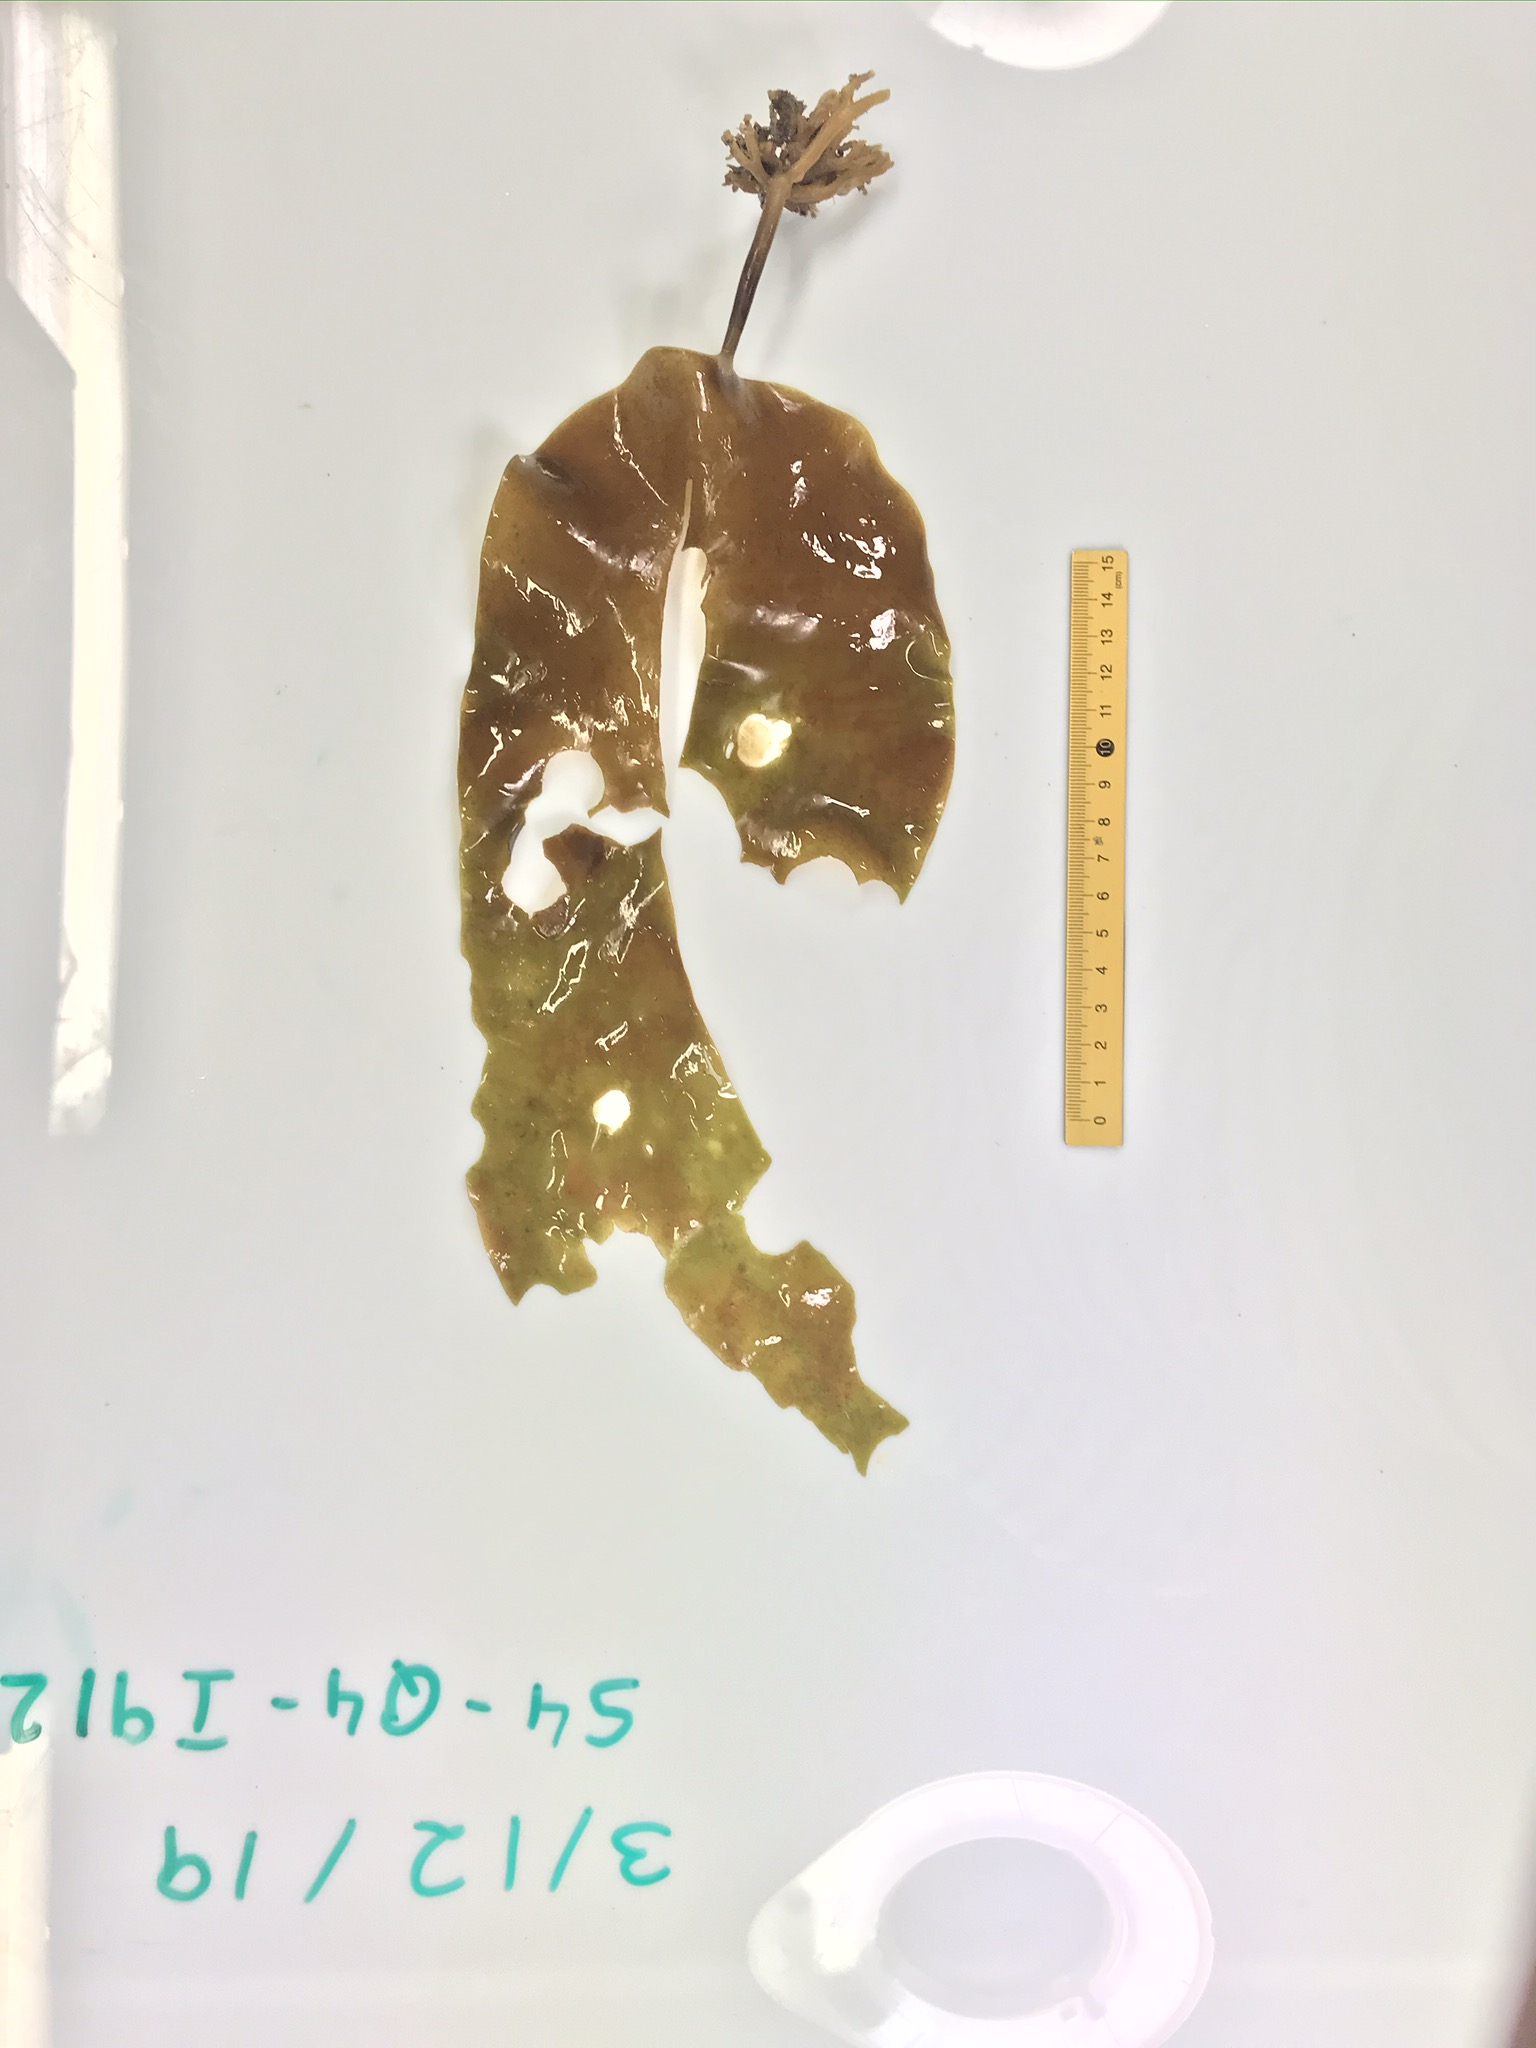
\includegraphics[width=0.32\textwidth]{imaxes/Alga_exemplo_intro_1.JPEG}
    \hfill
    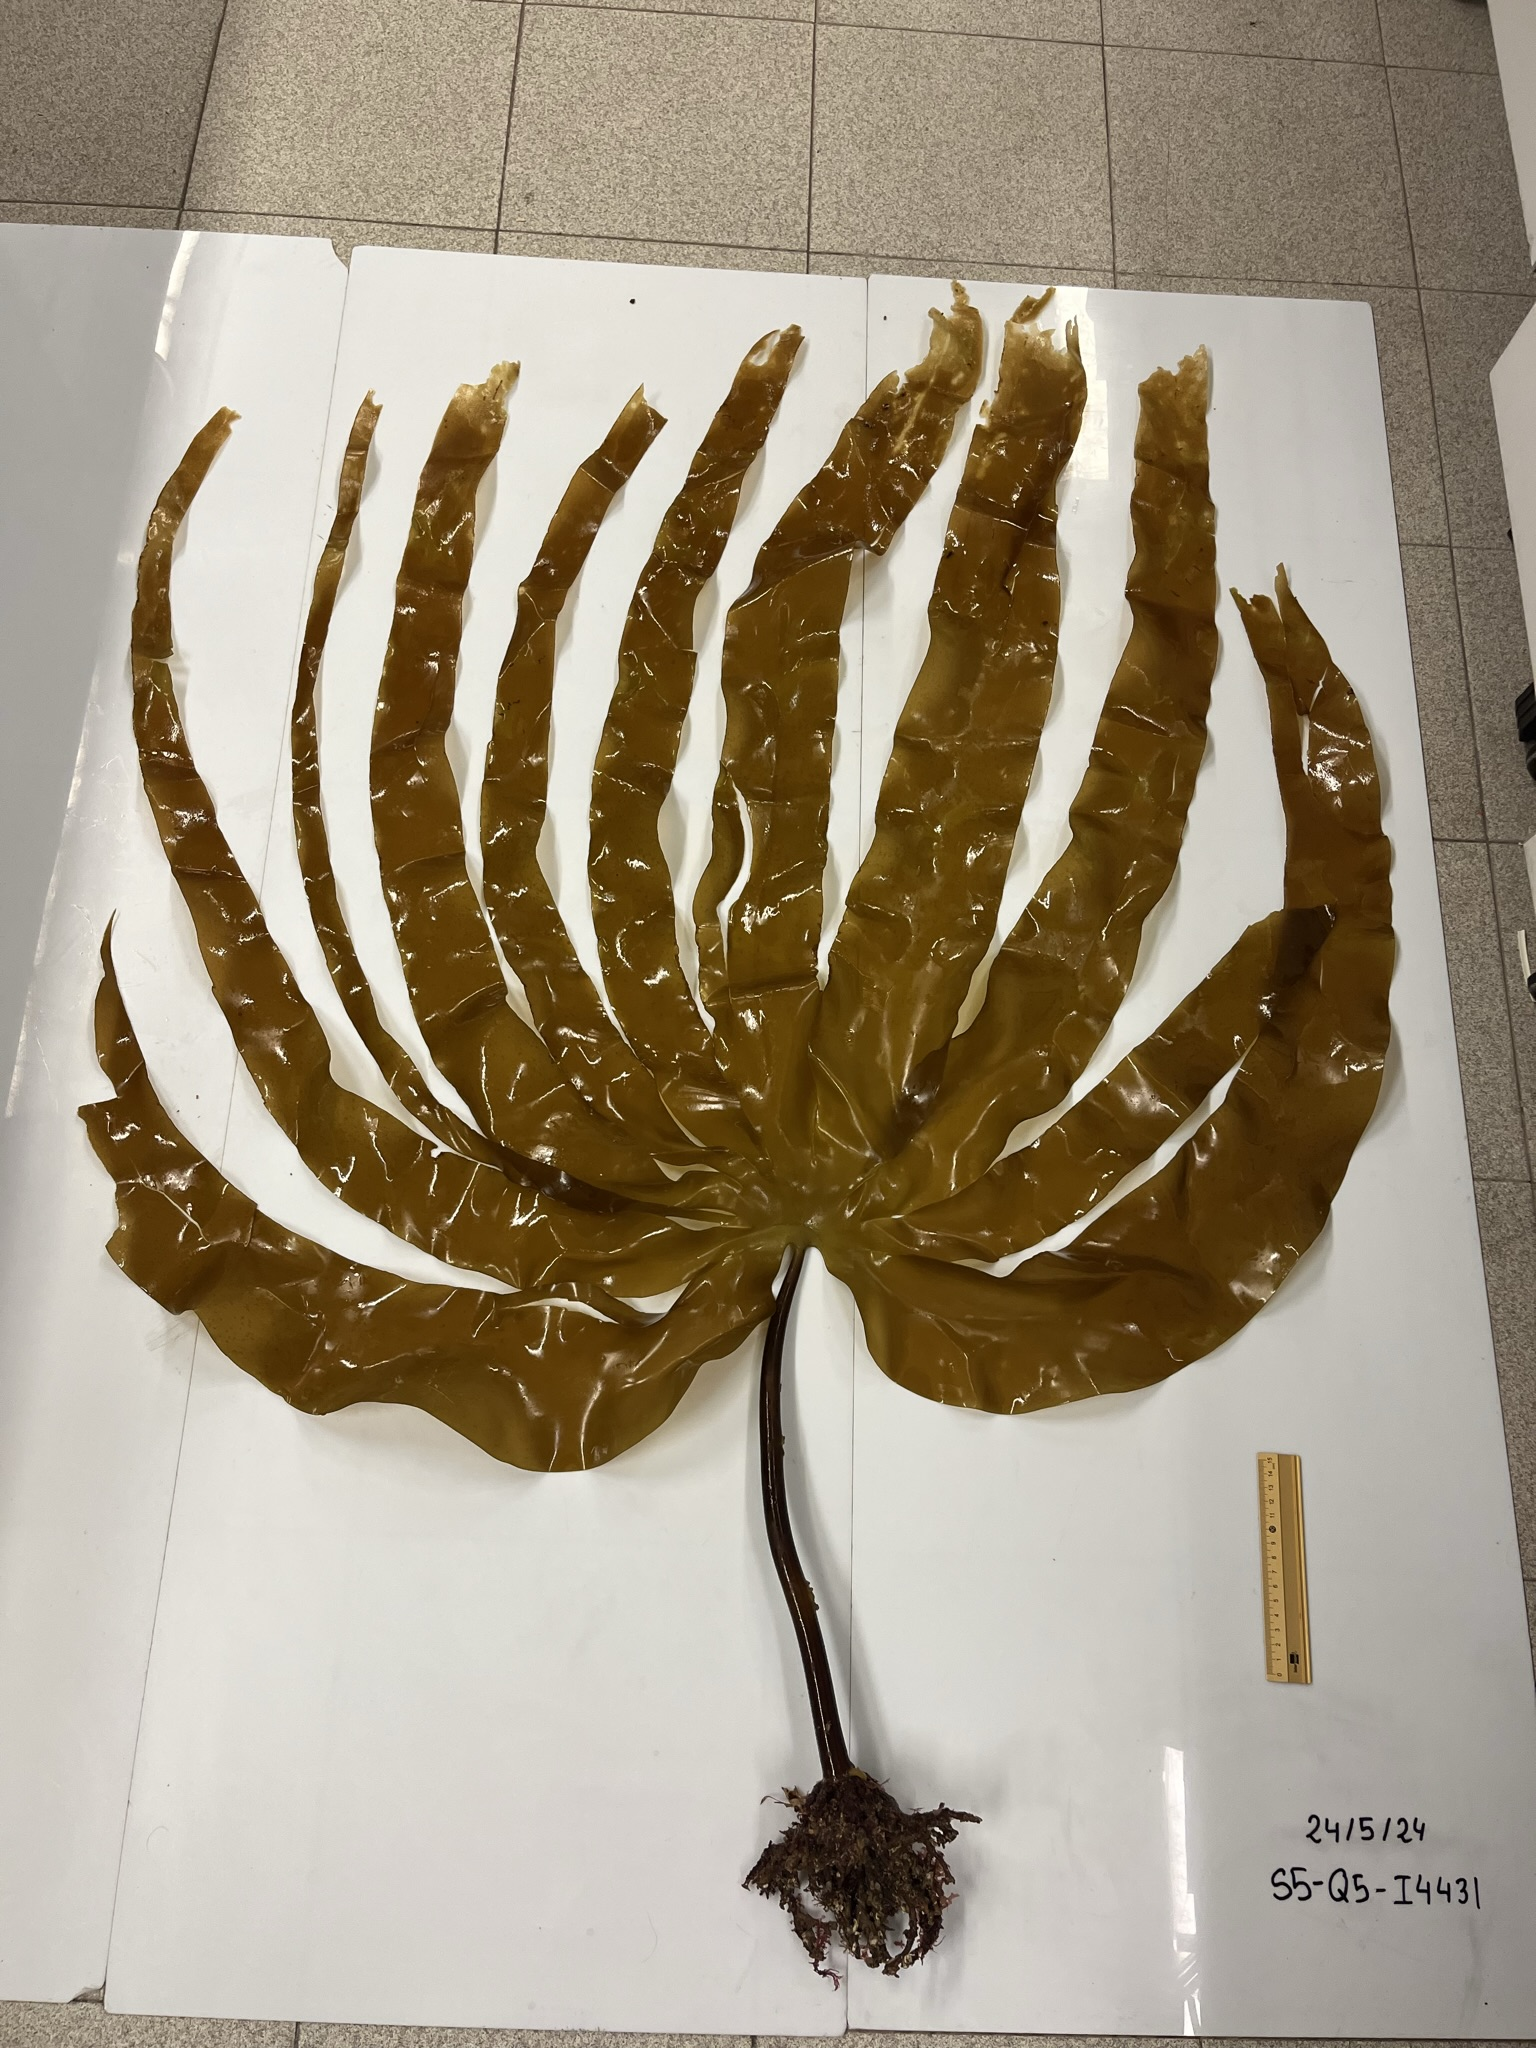
\includegraphics[width=0.32\textwidth]{imaxes/Alga_exemplo_intro_2.JPEG}
    \hfill
    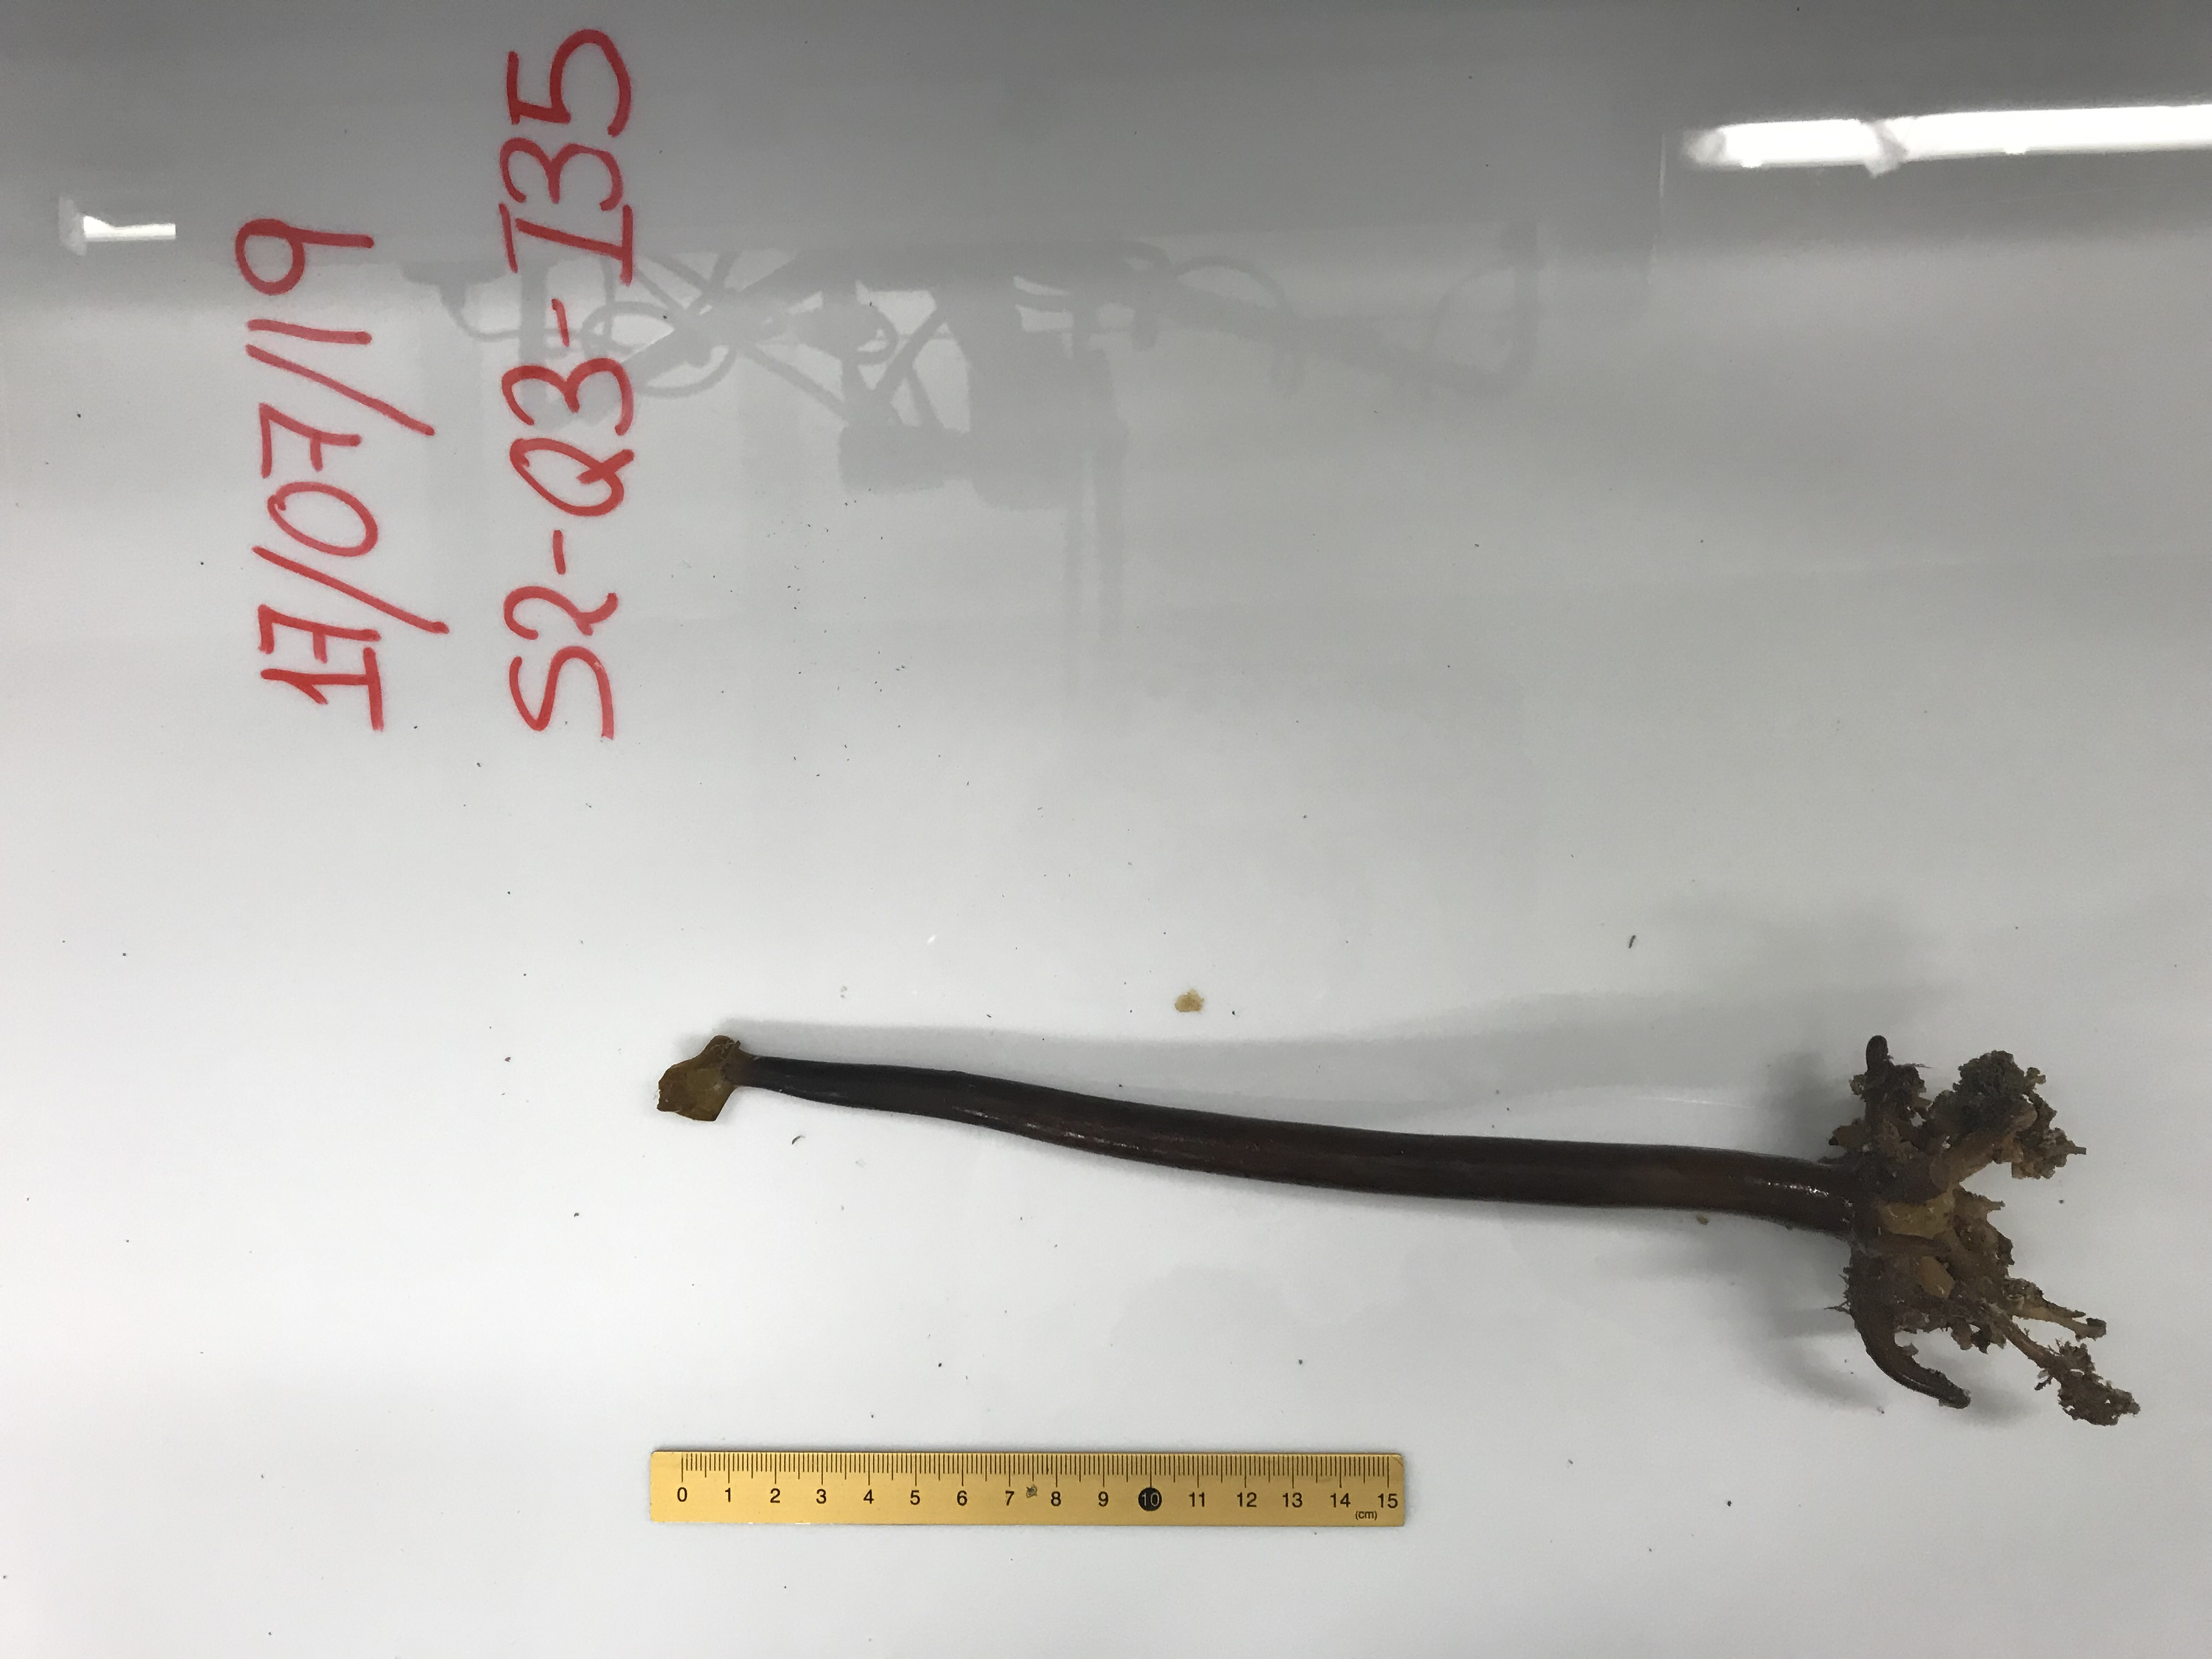
\includegraphics[width=0.32\textwidth]{imaxes/Alga_exemplo_intro_3.JPG}
    \caption{Exemplos variados de imaxes do \textit{dataset} empregado.}
    \label{fig:irregularidades-dataset}
\end{figure}

Todo isto fai necesaria a división do sistema en varias etapas. En primeiro lugar, precísase un
preprocesado das imaxes que permita estandarizar, na medida do posible, o \textit{dataset} e
reducir a influencia de variacións alleas ao fenómeno de interese, que poderían afectar ao
comportamento da \gls{cnn}. En segundo lugar, emprégase a propia \gls{cnn} para realizar a
inferencia sobre as imaxes tomadas polos expertos e determinar tanto o nivel de dano da alga como a
orixe da depredación. De aquí en adiante, referirémonos a estes valores como \gls{hpi} e
\gls{ivr}, respectivamente. Esta é a nomenclatura empregada polos biólogos no \textit{dataset}
proporcionado.

Finalmente, resulta necesario deseñar unha \textit{pipeline} que encapsule estes procesos e
simplifique o uso do sistema por parte dos expertos. Deste xeito, os biólogos unicamente terán que
incorporar unha imaxe ao programa, que lles devolverá a inferencia da \gls{cnn} como apoio á súa
toma de decisións.
 
\section{Obxectivos}

\subsection{Obxectivo xeral}
De forma global, este traballo pretende desenvolver un programa informático que poida asistir aos biólogos 
na clasificación e cuantificación de danos causados a algas Laminarias, buscando un sistema que priorice 
a exactitude na inferencia e a facilidade de uso.

\subsection{Obxectivos específicos}

\begin{itemize}
    \item Analizar e preparar o conxunto de datos dispoñibles para o problema.
    \item Deseñar unha etapa de preprocesado que reduza a variabilidade e normalice as imaxes atopadas no conxunto de datos.
    \item Desenvolver un modelo que proporcione unha inferencia para estimar as variables das algas (\gls{hpi}, \gls{ivr}).
    \item Integración do sistema nunha ferramenta usable polos expertos.
    \item Avaliar o comportamento do sistema con datos reais.
\end{itemize}


\section{Enxeñaría de desenvolvemento}

Desde o punto de vista da enxeñaría de desenvolvemento, o traballo organizouse como un proceso
iterativo e incremental. Nun primeiro momento dividiuse o problema global nas mesmas grandes fases
que estruturan esta memoria: análise do dominio e do conxunto de datos, preparación das imaxes,
detección e recorte das algas, normalización dos recortes, deseño dos modelos de aprendizaxe
profunda, avaliación experimental e integración final da \textit{pipeline}. Esta división permitiu
traballar sobre obxectivos máis acoutados e validar cada decisión antes de incorporala ao sistema
completo.

O desenvolvemento non seguiu unha secuencia estritamente lineal. Aínda que as fases principais se
presentan de maneira ordenada, en varias ocasións foi necesario volver sobre decisións previas a
partir dos resultados obtidos. Por exemplo, a primeira análise dos recortes xerados automaticamente
serviu para detectar erros de segmentación e motivou unha etapa posterior de revisión e curación dos
datos. Do mesmo xeito, os resultados iniciais da \gls{cnn} levaron a reformular a saída do modelo,
comparar diferentes arquitecturas e introducir a lóxica experta asociada á aplicabilidade de
\gls{ivr}. Polo tanto, cada bloque do sistema foi refinándose mediante ciclos de implementación,
avaliación e corrección.

As primeiras semanas dedicáronse á comprensión do problema biolóxico, á revisión das variables
incluídas no \textit{dataset} e á identificación das dificultades presentes nas imaxes reais. A
partir desta análise abordouse a preparación dos datos: primeiro mediante unha limpeza inicial e,
posteriormente, mediante a detección automática da rexión ocupada pola alga con YOLO. Esta etapa
permitiu separar o problema de localización do problema de estimación do dano, reducindo a
variabilidade visual que tería que asumir directamente a rede de clasificación.

Unha vez obtidos os recortes, o esforzo centrouse na súa normalización e revisión. Esta fase foi
especialmente relevante porque o conxunto de datos non procedía dun protocolo de captura
completamente controlado, polo que existían diferenzas de iluminación, escala, orientación e fondo.
Tras dispoñer dun conxunto de entrada máis homoxéneo, desenvolvéronse as primeiras versións da
\gls{cnn}, preparáronse os particionamentos de adestramento, validación e proba, e comparáronse
distintas formulacións do problema.

Na parte final do traballo, o desenvolvemento concentrouse na mellora da estimación de \gls{hpi} e
\gls{ivr}, na análise dos erros máis frecuentes e na integración da solución nunha \textit{pipeline}
de inferencia usable. Finalmente, realizouse unha validación con expertas sobre un subconxunto de
imaxes, o que permitiu contrastar o comportamento do sistema co criterio humano e contextualizar as
limitacións observadas.

\begin{figure}[htbp]
    \centering
    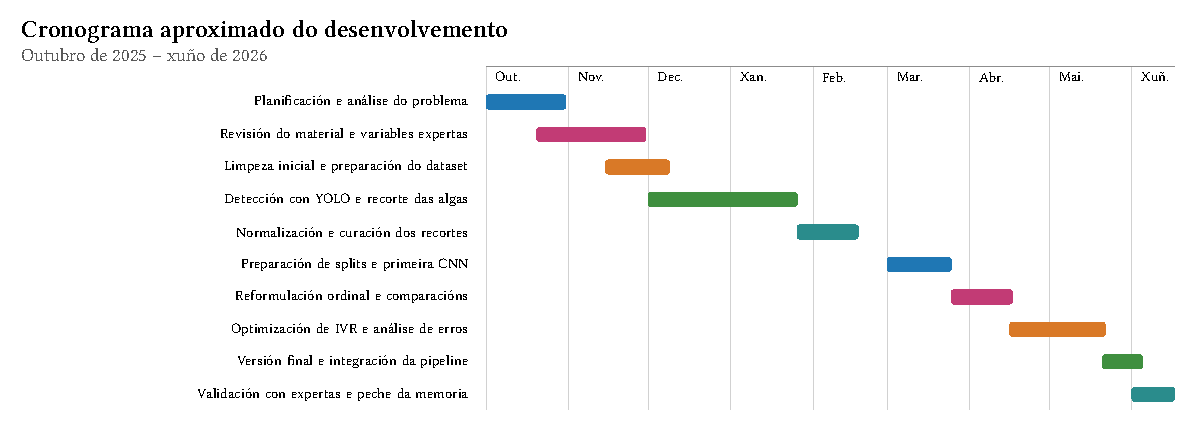
\includegraphics[width=\textwidth]{imaxes/cronograma_gantt.pdf}
    \caption{Cronograma aproximado das principais fases de desenvolvemento do traballo.}
    \label{fig:cronograma-gantt}
\end{figure}

Na Figura~\ref{fig:cronograma-gantt} móstrase a planificación temporal aproximada seguida durante o
proxecto. O solapamento entre varias tarefas reflicte precisamente o carácter iterativo do proceso:
mentres unha fase se pechaba, os resultados obtidos condicionaban axustes nas fases anteriores ou
servían de entrada para a seguinte iteración.
